% TEMPLATE for Usenix papers, specifically to meet requirements of
%  USENIX '05
% originally a template for producing IEEE-format articles using LaTeX.
%   written by Matthew Ward, CS Department, Worcester Polytechnic Institute.
% adapted by David Beazley for his excellent SWIG paper in Proceedings,
%   Tcl 96
% turned into a smartass generic template by De Clarke, with thanks to
%   both the above pioneers
% use at your own risk.  Complaints to /dev/null.
% make it two column with no page numbering, default is 10 point

% Munged by Fred Douglis <douglis@research.att.com> 10/97 to separate
% the .sty file from the LaTeX source template, so that people can
% more easily include the .sty file into an existing document.  Also
% changed to more closely follow the style guidelines as represented
% by the Word sample file. 

% Note that since 2010, USENIX does not require endnotes. If you want
% foot of page notes, don't include the endnotes package in the 
% usepackage command, below.

% This version uses the latex2e styles, not the very ancient 2.09 stuff.
\newcommand{\midtilde}{\raise.17ex\hbox{$\scriptstyle\mathtt{\sim}$}}
\documentclass[letterpaper,twocolumn,10pt]{article}
\usepackage{usenix,epsfig,endnotes,verbatim}
\begin{document}

%don't want date printed
\date{}
%make title bold and 14 pt font (Latex default is non-bold, 16 pt)
\title{\Large \bf The Effect of Virtualization in Timing the Ext2 File System}
%for single author (just remove % characters)
\author{
{\rm Rob Jellinek}\\
\and
{\rm Adam Vail}\\
} % end author

\maketitle
% Use the following at camera-ready time to suppress page numbers.
% Comment it out when you first submit the paper for review.
\thispagestyle{empty}

\subsection*{Abstract}
In this paper, we perform experiments to determine four characteristics of the ext2 file system in both a native Ubuntu 12.04 setting, and on a virtual machine using QEMU-KVM with virtio and running Ubuntu 12.04 as a guest. The experiments aim to determine the ideal buffer size for random file access, the amount of data prefetched by the file system during a sequential read, the size of the file cache, and the file size above which the file system adds a layer of indirection. We show that the ideal buffer size for random file access is 4096 bytes, that ext2 prefetches 128 KB of data, that the file cache is roughly 5.3 GB for 6 GB of memory, and that ext2 adds a layer of indirection for files greater than 48 KB. While our experimental results in the native and virtual settings were in agreement, the read and write latency on the virtual machine was almost always longer than in the native setting.

\section{Introduction}

In recent years large and small businesses have demanded cost effective ways of increasing their computing power.
This has led to the proliferation of full hardware virtualization.
Virtualizing computing resources has revolutionized the current environment in two distinct ways.
It has allowed companies to fully utilize their current systems by consolidating many machines onto a single physical system.
It has also produced new business models where companies flexibly rent computing time to customers who can pay for only what they need.

In order to run unaltered commodity operating systems, the virtual machine monitor must fully virtualize the system's underlying hardware.
This leads to a question of what performance differences arise when software that assumes it is running directly on bare hardware is run in a virtualized environment?
Therefore, we examined the effects of virtualization on the ext2 file system.
We studied four specific characteristics of ext2, comparing its performance when running on bare metal and when running in a virtual machine.

The first characteristic that was measured was the ideal buffer size when randomly reading from a file. 
The experiment tested different buffer lengths at different increments. 
It was determined that for both bare metal and virtual, buffers under 4096 bytes in size perform similarly when randomly reading from a file. 
Buffers over 4096 bytes in size require an increase in cycles to read all the data. 
This buffer size represents the block size for the file system. 
When ext2 reads and writes to disk it does so at the block level.
Blocks are a foundational element in file systems and this value is significant because it is then used in all other file system measurements.

The second characteristic measured was the amount of data prefetched by the file system. 
When reading from a disk, the file system assumes the user will most likely read data sequentially. 
In order to increase performance for this common case the file system reads extra blocks that are located after the requested data. 
This is useful because it allows the user to read sequentially without constantly paying the penalty for having to go out to disk. 
Again, the experiment yielded results indicating that ext2 behaves similarly in both environments, prefetching 128 KB of data whenever a block is read from disk.

The third characteristic measured was the size of the file system cache. 
This is particularly important to the user since it indicates the amount of data that they can access without incurring large delays. 
It is not a uniform characteristic across all instances of ext2 since the size is related to the amount of free memory in the system.
Both the bare metal and virtual machine were equipped with 6 GB of memory which in both cases yielded a cache size of about 5.3 GB. 

The final characteristic measured was the file size at which ext2 requires indirection to store data. 
Since ext2 uses inodes to organize data on disk, the number of pointers in the inode that directly reference data determines the largest file size before needing to use indirection. 
Then, extra layers of indirection are used as the file size increases. 
Ext2 implements three levels of indirection which allows for file sizes up to 2 TB (depending on the block size). 
The experiment showed that in both settings ext2 uses twelve direct inodes. 
Therefore, an inodes can directly reference a file of up to 48 KB. 

While the boundaries at which the file system operated were very similar in both environments, the virtual environment incurred extra delay in every experiment.
This is not surprising due to the fact that all operations in the virtual environment had to go through a hypervisor.

\section{Methodology}
\subsection{Environment}
All experiments, both on bare metal and virtualized, were run using 64-bit Ubuntu 12.04 (Linux 3.2.0-30-generic kernel) and the ext2 file system.
The system used an Intel Core i5 2.8 GHz quad-core processor with Intel VT enabled.
Virtualization was done via KVM (Kernel-based Virtual Machine) which offers full virtualization of the x86 hardware.
KVM was configured to use virtio to virtualize all I/O operations.
The virtual machine was given a single processor.
The test machine was equipped with 6 GB of memory for all bare metal experiments.
In order to allow the virtual machine to also have 6 GB of memory, 12 GB of memory was installed in the test machine when running the virtual experiments.
All experiments were implemented in C, run multiple times, and were run identically between the bare and virtual environments.
The cache was dropped between runs of every experiment using the \texttt{drop\_caches} ability provided by the kernel.
The ext2 file system was on a SATA connected 500 GB Western Digital Caviar Green drive. 
The Caviar Green family of disks adjusts the speed of the drive in order to save power. 
This power saving mode goes into effect after eight seconds of inactivity.
The first run of every experiment was used to "wake up" the drive and was subsequently thrown out due to needing "spin-up" time. 

The timer used for all experiments was the time stamp counter, accessed through the \texttt{rdtsc} instruction provided by the Intel instruction set. 
The command allows access to the cycle count which was used to determine how many cycles it took for an operation to complete. 
This does have the potential to introduce some noise since the CPU is not restricted to run at a fixed frequency. 
Discarding the first run of every experiment helps minimize this inconsistency. 
The timer was tested against the \texttt{gettimeofday()} function. 
The test program slept for several seconds and both the time stamp counter and \texttt{gettimeofday()} determined the same amount of sleep time. 
Although, each core in a multi-core processor has its own time stamp counter.
Therefore, the experiments were run with the \texttt{taskset} and \texttt{nice} commands in order to affinitize the experiment to a single CPU and set its priority as high as possible.

\subsection{Measuring the Ideal Buffer Size for Random Reads}

In order to determine the ideal buffer size when performing random reads, reads of various sizes were performed and the times for each read were compared. 
Since this measurement is essentially determining the block size, if bytes are read from the same block then they should have fast access times. 
Once the file system needs to read from a new block it will have to fetch that block before returning the data. 
Therefore, when the read time increases significantly it is the start of a new block.
Reads were started from a block chosen randomly within the first 1000 blocks of the file and were done in reverse order to counteract prefetching. 
Since the default page size for the Linux kernel is 4 KB, it is logical that the file system make this its basic unit for moving data. 
Therefore, we expected the ext2 block size to be 4096 bytes.

\begin{verbatim}
    // step: amount of bytes 
    // to skip between reads
    // was varied, all 
    // yielding same results
    int step = 512  
    int i = 0;
    for(i; i <= 20; i++){ 
        buffer = (char *)malloc(1);
        lseek(fd, 
          base - (i * step), SEEK_SET);
        time_start = rdtsc();
        read(fd, buffer, 1);
        time_stop = rdtsc();
        free(buffer);
    }
\end{verbatim} 

\subsection{Measuring the Amount of Data Prefetched by the File System}
When a block is read from the disk the file system makes the assumption that the data following that block is going to be read in the near future. 
Thus, when a block is read, some number of subsequent blocks are cached so that when the application reads these blocks they can be returned much faster than going out to disk. 
The experiment randomly chose a block to read from the first 1000 blocks of the file. 
It then slept for one second in order to allow for all the prefetched data to be put into the cache. 
It then sequentially read the blocks following the initial block and timed how long it took for that block to be read. 
Blocks in the cache should be returned very quickly. 
A long read time for a block indicates that the file system had to go out to disk in order to retrieve it. 
Along with retrieval of that block the file system would again prefetch data. 
Therefore the expected timing distribution was a consistent number of fast reads (blocks in the cache) separated by spikes indicating the file system had to go out to the disk. 
The number of blocks from one spike to the next revealed the size of the prefetch.

\begin{verbatim}
    #define BLOCK 4096

    int i = 1;
    for(i; i <= 200; i++){
            time_start = rdtsc();
            read(fd, buffer, BLOCK);
            time_stop = rdtsc();
    }
\end{verbatim}

\subsection{Measuring the Cache Size}
The cache allows the file system to keep recently accessed (and potentially soon to be accessed due to prefetching) data in memory. 
By not having to go out to disk on a request it speeds up the retrieval time immensely. 
The size of the cache is affected by the amount of free physical memory in the system. 
The system we used for our experiments had two 6 GB DIMMs. 
In order to speed up test times and to provide a similar environment for the native and virtual settings, we removed a DIMM from the test machine for our bare metal tests, so that the machine was running on a total of 6GB of physical memory. 
In our VM-based tests, we inserted both DIMMs so that the machine had 12GB of physical memory, but only made 6 GB available to the virtual machine. 
Otherwise, with only one DIMM installed for the VM tests, we would have been unable to allocate the full 6 GB to the guest VM.
%Both the bare metal system as well as the virtual machine had 6 GB of memory and no extra applications running. 
We also consider that there is a source of noise in that operating system processes were running at the time of the experiments, thus taking up some amount of memory.
The experiments were run in a consistent environment in order to try and control the noise as much as possible. 
With 6 GB of memory it was expected that the cache would take up the majority of the free space and have a size near 5 GB. 
This was tested by doing repeated reads to the same blocks of data. 
Blocks in the cache have very fast read times. 
Once the amount of data being read is too large to fit inside the cache, the read times increase as the file system has to continually go out to disk due to cache misses. 
Prefetching was controlled by reading all the desired blocks initially without timing to allow for the data to be placed in the cache. 
Then, the same data was read again while being timed. 
All individual reads were of block size in order to avoid allocating large amounts of space on the heap and unnecessarily consuming memory.

\begin{verbatim}
    int step = 64
    int i = 1;
    for(i; i <= 190; i++){
        buffer = (char *)malloc(BLOCK);
        lseek(fd, 0, SEEK_SET);
        int k = 0;
        for(k; k < (long)step*i*MB/BLOCK; 
            k++){
                read(fd, buffer, BLOCK);
        }
        sleep(1);
        k = 0;
        lseek(fd, 0, SEEK_SET);
        time_start = rdtsc();
        for(k; k < (long)step*i*MB/BLOCK; 
            k++){
                read(fd, buffer, BLOCK);
        }
        time_stop = rdtsc();
        free(buffer);
    }
\end{verbatim}

\subsection{Inode Indirection}
%% TODO once we figure out what is going on here
Ext2 uses inodes in order to organize data on disk. 
Since many files are relatively small, inodes can reference a handful of blocks directly before resorting to single, double, or triple indirection.
The number of directly referable data blocks can be determined by writing a single block to disk and measuring the amount of time it takes. 
The operating system does some optimizations when writing data to disk, such as batching, due to its cost. 
Because of this, each block must be flushed out to disk by the \texttt{fsync} command.
Eventually the direct pointers will be exhausted and a level of indirection will be used. 
This causes two separate writes. 
First the indirect pointer, and then the actual pointer to the data. 
This is then followed by the write for the actual block. 
Having to complete two writes causes the time needed to complete the operation to spike. 
Therefore, a spike in write time indicates the use of indirection.
Since both the bare metal and virtual machine are using ext2, and ext2's documentation states that it supports twelve direct references to data blocks, we expect that both environments allow a file up to 48 KB to be directly referenced by the inode.

\begin{verbatim}
    int i = 0;
    for(i; i < 16; i++){
            time_start = rdtsc();
            write(fd, buffer, BLOCK);
            fsync(fd);
            time_stop = rdtsc();
    }
\end{verbatim}

\section{Results}

\subsection{Buffer Size}
\begin{figure}[!ht]
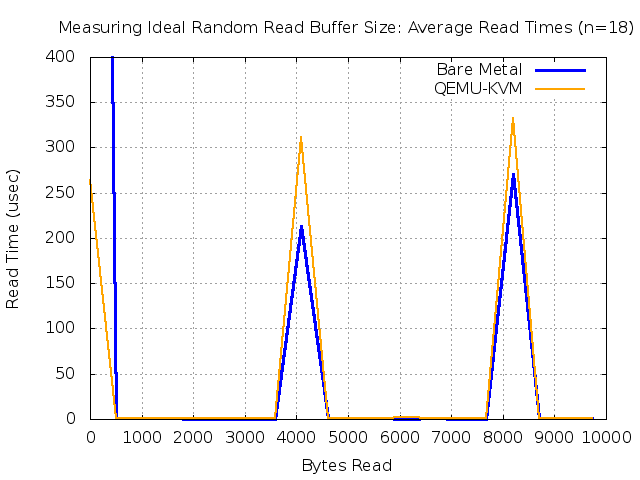
\includegraphics[scale=.35]{combined_graphs/random_avg.png}
\caption{Ideal buffer size for random file access: average read times. Reads take longer on 4096-byte boundaries, indicating that this is the size of a block, and is the optimal buffer size for random reads.}
\end{figure}
\begin{figure}[!ht]
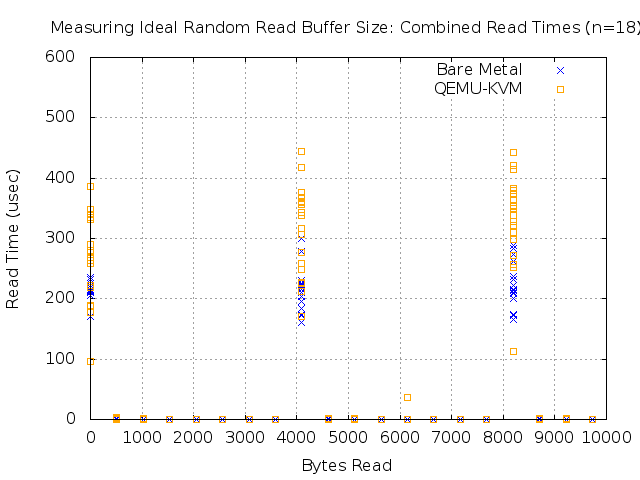
\includegraphics[scale=.35]{combined_graphs/random_combined.png}
\caption{Ideal buffer size for random file access: combined read times}
\end{figure}

When reading single bytes in reverse starting from a random point in our target file on ext2, read times jumped on 4096-byte boundaries. 
On bare metal, average read times jumped from approximately 0.5 microseconds when the read happened within a 4 KB block, to 200-250 microseconds for the first read into a new 4 KB block. 
Under QEMU-KVM, read times within a block took approximately 0.75 microseconds and jumped to 300-400 microseconds for the first read into a new 4 KB block.  

This is consistent with our hypothesis that read times would spike on the first read into a new block but remain low otherwise. 
Since ext2 defines a block size as 4096 bytes, the first read into a new block fetches the block from disk into memory; all subsequent reads from that block can be done directly from memory, and so are much quicker.

The consistency in spikes but relative difference in latency between our bare-metal and QEMU-KVM tests are also consistent with our expectations. 
Virtio implements virtual queues that serve as an interface between a set of front-end drivers in QEMU, and back-end drivers in the KVM hypervisor. 
I/O requests and responses are passed between guest and host first via the virtio-blk device driver and then through these queues to the hypervisor, where the actual I/O request is then made and the result is returned to the guest. 
The additional time required to transfer the I/O request and response would explain the higher response time observed under QEMU-KVM when compared with bare metal. 
In particular, the greater relative slowdown when a block is newly fetched from disk (\midtilde100 microsecond difference between bare metal and VM), compared with when data is fetched from memory (\midtilde0.25 microsecond slowdown for the VM) is in line with expectations. 

\subsection{Prefetching}
\begin{figure}[!ht]
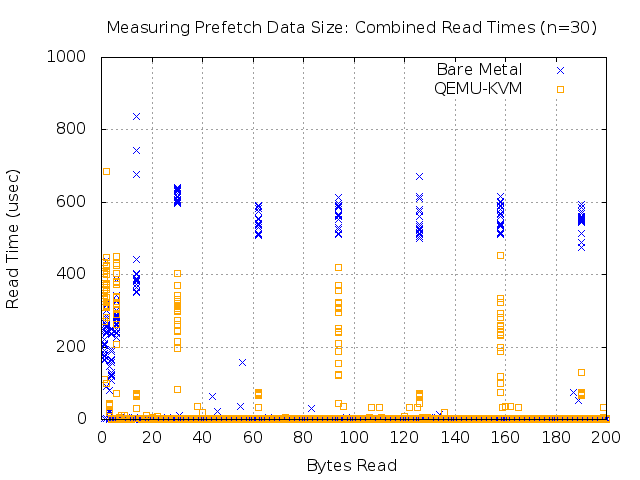
\includegraphics[scale=.35]{combined_graphs/prefetch_combined.png}
\caption{Measuring sequential reads to determine prefetching size: combined read times. Read latency spiked every 32 blocks, indicating that ext2 prefetches 128 KB of data.}
\label{fig:prefetch_combined}
\end{figure}
Our results in Figure \ref{fig:prefetch_combined} confirmed our hypothesis that read times on a sequential read would be fast over some set number of blocks, indicating that those blocks were resident in memory due to prefetching, and would spike when the next set of blocks had to be read from disk. 
Our results show that the high read times occur at 32-block intervals, indicating that ext2 prefetches 128 KB of data at a time. 

Read times from memory were roughly 1 microsecond in both the native and virtual settings, and jumped to approximately 600 microseconds in both settings, though the highest read latencies observed were on the VM. 
This makes sense, since all else being equal (in particular, assuming the virtualization layer is not doing any additional prefetching itself), reading from disk should take slightly longer for the VM due to the overhead added by virtio, as discussed in the previous section.

Initially our results indicated that the VM was able to prefetch much faster than the bare metal machine. 
We used \texttt{iostat} to monitor the amount each machine had to go out to disk to complete our experiment. 
We found that the VM had to make ten less trips to disk on average than the bare metal machine.
Therefore, KVM must do some amount of preemptive prefetching optimizations.
In order to control this setting, KVM was configured to use its native I/O mode which yielded the results shown above.
These results are in line with what one would expect when having to interact with a hypervisor.

\subsection{File Cache}
\begin{figure}[!ht]
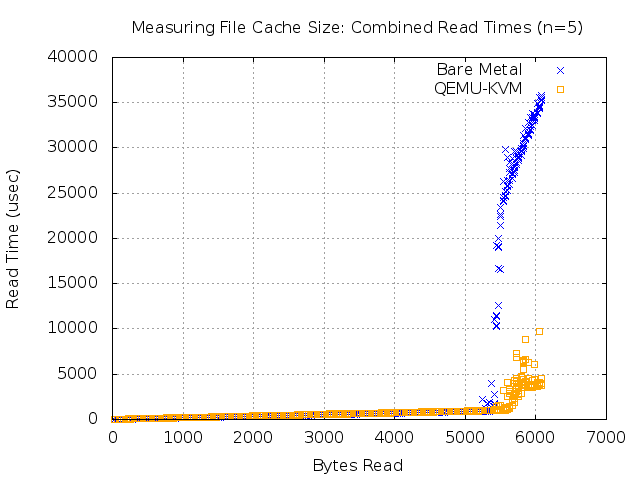
\includegraphics[scale=.35]{combined_graphs/cache_combined.png}
\caption{Measuring file cache size: combined read times. ext2 grows the file cache to fill available physical memory, and shrinks as more memory is used. With 6 GB of total physical memory, roughly 5.3 GB was available for the file cache.}
\label{fig:file_cache}
\end{figure}
Figure \ref{fig:file_cache} shows the results from our cache-timing tests in the native and virtual settings. 
Both settings show very low read times for the first 5.3 GB of data, implying that the data read in fit inside the file cache. 
We can assume that the remaining physical memory was consumed by background processes and kernel data structures. 
After the first 5.3 GB, the read time for additional bytes skyrockets in the native setting, but remains relatively low in the virtual setting. 
This is most likely attributable to our experimental setup, where we had only one 6 GB DIMM in the native setting, but two 6 GB DIMMs in the virtual setting (though we only allocated the 6 GB to the VM). 

%TODO: Is the following correct or plausible? Potentially talking out my a**. Especially toward the end.
In the native setting with 6 GB of physical memory, assuming the file cache was 5.3 GB and background processes and the kernel filled the remaining space, no additional files could be cached in physical memory past the 5.3GB mark. 
This makes sense, as we know the size of the file cache is dependent on the amount of free physical memory in the system at the given time. 
In this case, it filled almost all the free physical memory. 
Reading additional files would require going to disk in each case, swapping out old data from the cache, and replacing it with the new data read, all of which is very expensive. 
In the VM setting, however, since we actually have 12 GB of physical RAM, the VM will fill up its own file cache, which appears to be slightly larger than that from the native setting (probably because the bare Linux installation in the VM had fewer modules/background processes loaded). 
But then when it tries to read an additional file, it is cached in the remaining free physical memory of the hypervisor--outside the 6GB visible to the guest VM, but accessible now only with the overhead required to swap the page in from the hypervisor's memory into the guest OS's memory. 
If read pages are shared, this may not even involve a swap, but only a page-table update. 

\subsection{Inode Indirection}
\begin{figure}[!ht]
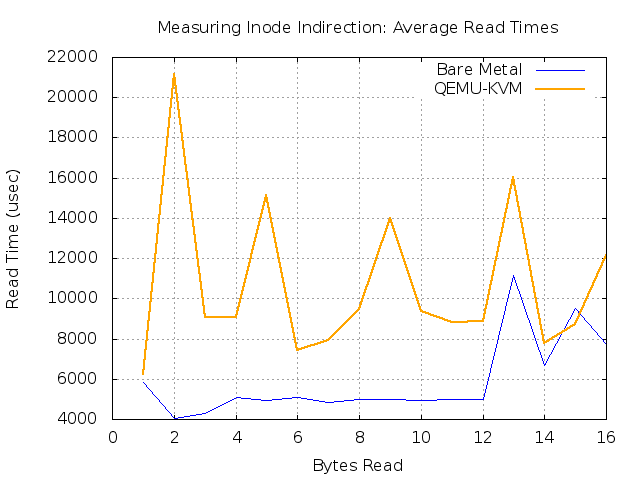
\includegraphics[scale=.35]{combined_graphs/inode_avg.png}
\caption{Measuring sequential write latency to determine inode indirection: average write times. The spike in write latency at the 13th data block implies that the first 12 blocks are pointed to from direct pointers, while the 13th block is pointed to from an indirect pointer, which takes additional time load and write.}
\label{fig:inode_avg}
\end{figure}
%\begin{figure}[!ht]
%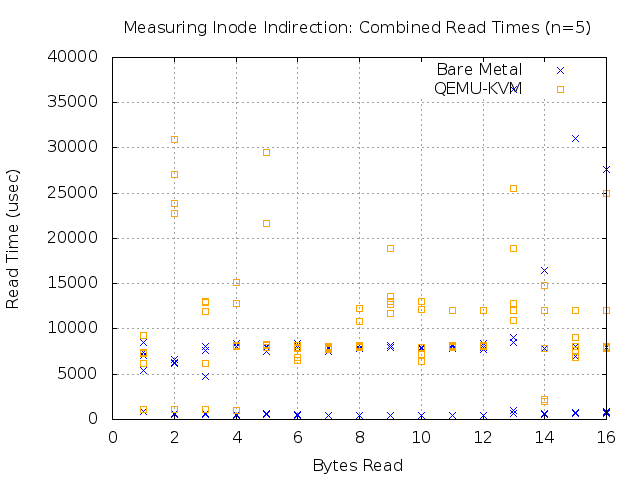
\includegraphics[scale=.35]{combined_graphs/inode_combined.png}
%\caption{Measuring sequential write latency to determine inode indirection: combined write times}
%\label{fig:inode_combined}
%\end{figure}
An ext2 inode contains a handful of direct pointers to data blocks, followed by single, double, and triple indirect pointer blocks.
By timing sequential block-sized writes we can determine the number of direct pointers in the inode itself.
If the block is referenced directly then only the direct pointer must be written.
If the block is referenced indirectly, then the indirect pointer and the direct pointer must be written.
The need to complete two writes instead of one causes an increase in write time once the file is above a certain size.

This pattern is visible in both the native and virtual environments as seen in the timings in Figure \ref{fig:inode_avg}. % and \ref{fig:inode_combined}. 
We see a spike in read times from roughly 5 ms to 11 ms on bare metal, and 8 ms to 21 ms on the VM, which indicates that there are 12 direct pointers in an ext2 inode, and the 13th is an indirect pointer. 
Upon writing the 13th data block the file system wrote the indirect pointer, followed the pointer, and wrote the direct pointer before writing the desired data.
This adds an additional operation to the \verb~write()~ over those performed using the first 12 direct pointers. 
Since each direct pointer points to a 4096-byte data block, the file system adds an additional layer of indirection for files over 48 KB in size.

As in our other experiments, the additional delay of the VM over the native setting makes sense given that the hypervisor has to perform the same write as in the native setting, and additionally incurs the overhead associated with processing the request through virtio.

We faced several issues in timing inode indirection in both the bare metal and virtual environment.
In both cases our initial results showed widely varying times for all writes to a file.
We again used \texttt{iostat} to inspect how often the machines were going to disk during the experiments.
In the bare metal environment, it was observed that the system went to disk several times in the five seconds directly after our experiment would run.
These extra writes would then interleave with the next run of our experiment causing the disk head to start from different places.
Thus, when timing block writes, each write would incur some amount of seek time that varied depending on the interleaving.
To counteract this, we delayed consecutive runs of our experiment by 5 seconds to allow the system to return to a state where it wasn't writing to disk.

In the virtual environment \texttt{iostat} showed that the machine was almost constantly talking to disk, causing similar problems.
We used \texttt{iotop} to inspect which process was making the writes and discovered that KVM has a \texttt{flush} process that frequently writes out to disk.
In order to limit this process we configured KVM's cache setting to \texttt{none} while running the inode experiments.

\section{Conclusions}
The preceding experiments have demonstrated that the ideal buffer size for random file access is 4096 bytes (the size of a block in ext2), that ext2 prefetches 128 KB of data, that the file cache on our 6 GB of memory fills the remaining 5.3 GB of free memory, and that ext2 adds a layer of indirection for files greater than 48 KB. 
In general, reads and writes to disk in QEMU-KVM took longer than similar reads and writes on native Linux, which makes sense given that in the virtual setting the same reads and writes must happen at the hypervisor level as in native Linux, but must also be passed between the hypervisor and guest via virtio's virtual queues. 
This communication must necessarily incur an overhead, which will be visible in timing experiments unless the virtualization layer employs additional techniques to minimize or amortize that overhead. 

We also realized how difficult it can be to get clean, consistent data in these timing experiments.
It is very difficult to control the environment to ensure the timing of specific variables and not incorporating extraneous factors.
In the end we accomplished this by controlling noise in the system (due to background processes), clearing the cache correctly, pinning the tests to a single CPU, and investigating steps the virtualization layer might be taking that would affect timing. 

%{\footnotesize \bibliographystyle{acm}
%\bibliography{../common/bibliography}}

%\theendnotes

\end{document}







